\documentclass{article}
\usepackage[framed,numbered,autolinebreaks,useliterate]{mcode}
\usepackage{graphicx}
\graphicspath{ {images/} }
\usepackage{Sweave}
\begin{document}
\Sconcordance{concordance:test_tex.tex:test_tex.Rnw:%
1 4 1 1 0 13 1}



First I attached this part of map by ggmap. To run this tex file faster I just attach the picture rather than run the ggmap code in this tex file.\\
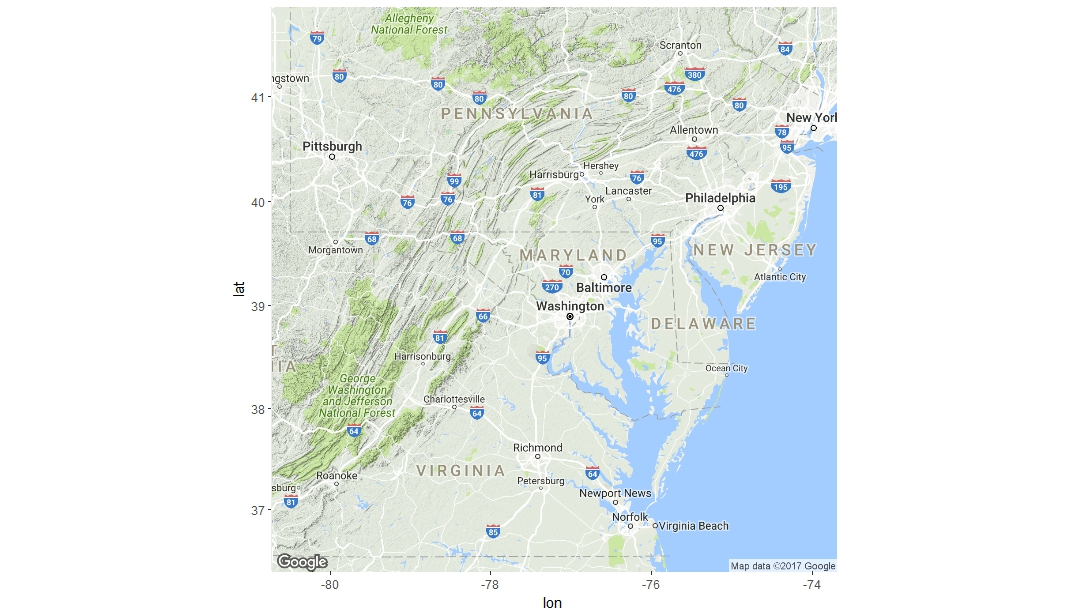
\includegraphics[width=15cm,height=15cm,keepaspectratio]{Rplot}\\
Now I have a contour plot from Matlab:\\
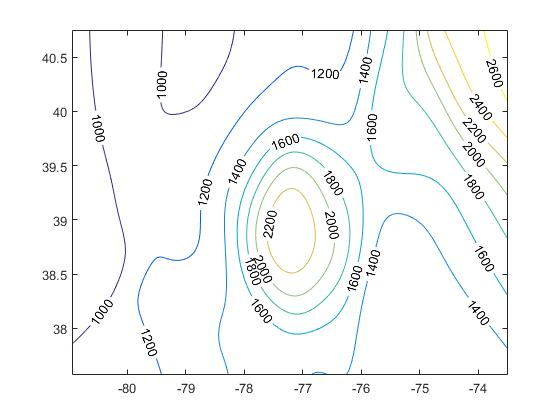
\includegraphics[width=15cm,height=15cm,keepaspectratio]{contour}\\
Which clearly shows that there are two peaks of ZRI on Washington D.C and New York.\\
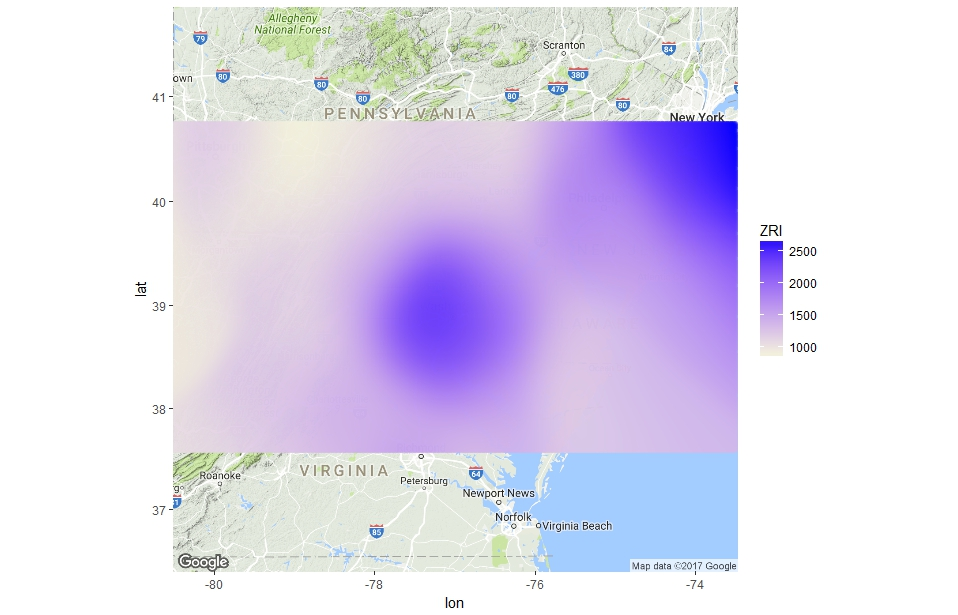
\includegraphics[width=15cm,height=15cm,keepaspectratio]{heatmap}\\
And finally a heat map generated by ggmap in R. It shows the same result.


\end{document}
